\section{Date necesare}
\paragraph{}
Datele de antrenament sunt extrem de importante.
O expresie populară\footnote{Expresia este ``garbage in, garbage out'', iar o expresie românească similară ar fi ``semeni vânt, culegi furtună''} ne spune că dacă datele furnizate algorimilor de învățare automată sunt de proastă calitate, atunci așa va fi și performanța acelor algoritmi, sau mai bine spus a modelelor matematice și a generalizărilor create de aceștia.
Mulțimea de date trebuie să conțină varietate, în cazul de față însemnând poze cu fundaluri diferite, condiții de iluminare diverse ș.a.m.d.

\paragraph{}
Am lucrat cu imagini cu utilizatorul, capturate prin webcam.
Apoi, am extras fie doar fața acestuia din imagine, fie doar un ochi, fie o porțiune rectangulară în care se regăsesc ambii ochi.
Pentru fiecare experiment realizat, am menționat ce date au fost folosite și în ce mod au fost procesate acestea.

% ========== Data Collection Section ==========
\section{Obținerea datelor}

\subsection{Moduri de obținere}
\paragraph{}
Pentru colectarea datelor am implementat 2 metode: o metodă ``activă'' și una ``pasivă''.
Folosind-o pe cea activă, utilizatorul trebuie să urmărească cu ochii cursorul mouse-ului în timp ce acesta se mișcă pe ecran prin mișcări glisante, de la stânga la dreapta, apoi de la dreapta la stânga, astfel încât să acopere toată suprafața ecranului.
De fiecare dată când s-a efectuat o mișcare a cursorului este capturată și o imagine și este salvată împreună cu poziția cursorului pe ecran la acel moment.

\paragraph{}
Metoda pasivă este menită să nu deranjeze rutina utilizatorului, astfel încât de fiecare dată când utilizatorul apasă pe butonul stâng al mouse-ului, aplicația salvează, în același mod ca mai sus, o imagine capturată prin intermediul webcam-ului și poziția cursorului pe ecran.
Este important de menționat că de multe ori nu ne uităm acolo unde apăsăm cu mouse-ul, așa că, deși este o metodă gândită să ruleze pe fundal, este bine ca utilizatorul să țină cont de prezența acesteia și să realizeze apăsări de buton acolo unde se uită, pentru a construi \emph{date consistente}.


\begin{lstlisting}[language=Python, caption=Colectarea datelor]
def start_collecting(self, collection_type):
    dc_logger.info(f'Start collecting data in {collection_type} mode')
    WebcamCapturer.start_capturing()
    self.gui.start()
    dc_logger.info('DataCollectorGUI started')
    if collection_type == 'background':
        self.mouse_listener.start_listening()
        dc_logger.info('Mouse listener started')
    elif collection_type == 'active':
        threading.Thread(target=self.start_active_collection).start()
\end{lstlisting}

\subsection{Salvarea datelor}
\paragraph{}
Când colectarea datelor este gata, acestea sunt salvate sub forma unei ``sesiuni''.
Fiecare sesiune este definită de numărul imaginilor care au fost capturate, de rezoluția ecranului și rezoluția webcam-ului.
Mai jos se poate observa structura directoarelor și modul în care aceste date sunt salvate, fără a aplica vreo modificare.

\begin{figure}[h]
    \centering
    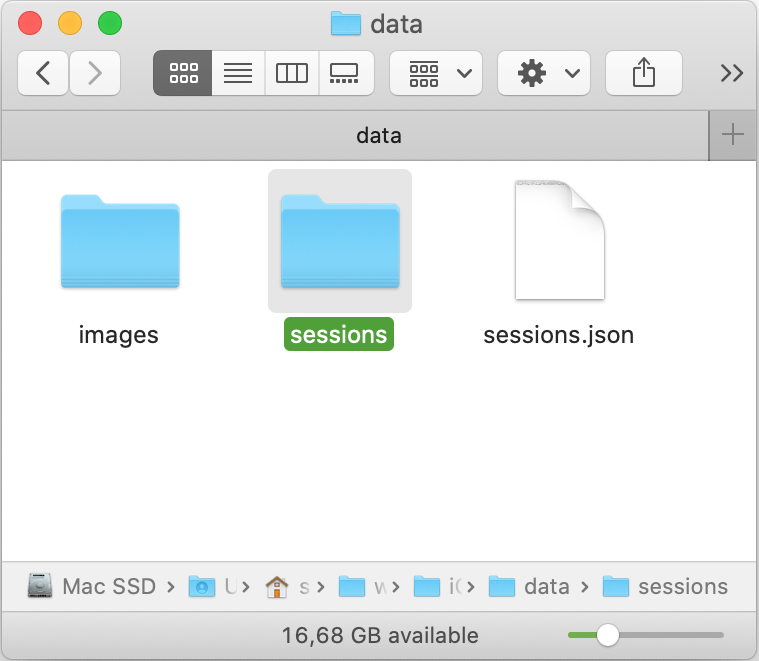
\includegraphics[width=0.3\textwidth]{data_structure_1.png}
    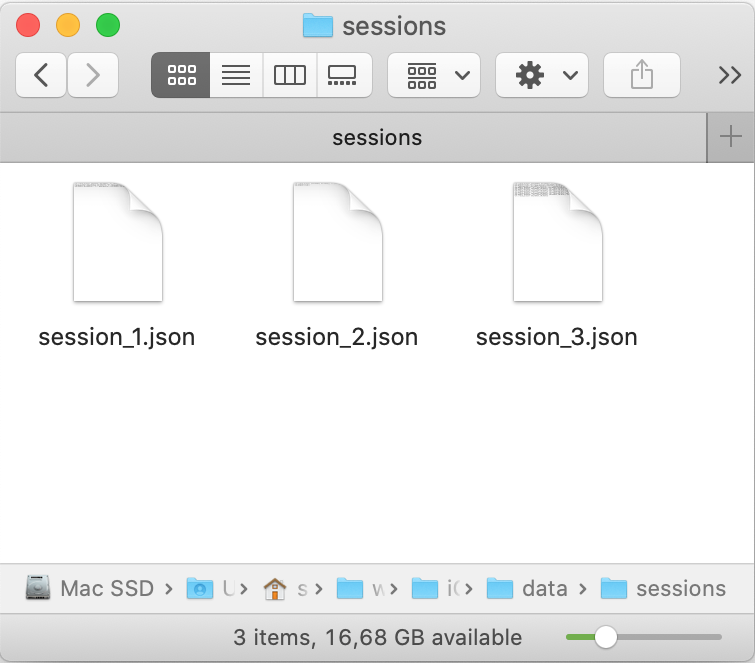
\includegraphics[width=0.3\textwidth]{data_structure_2.png}
    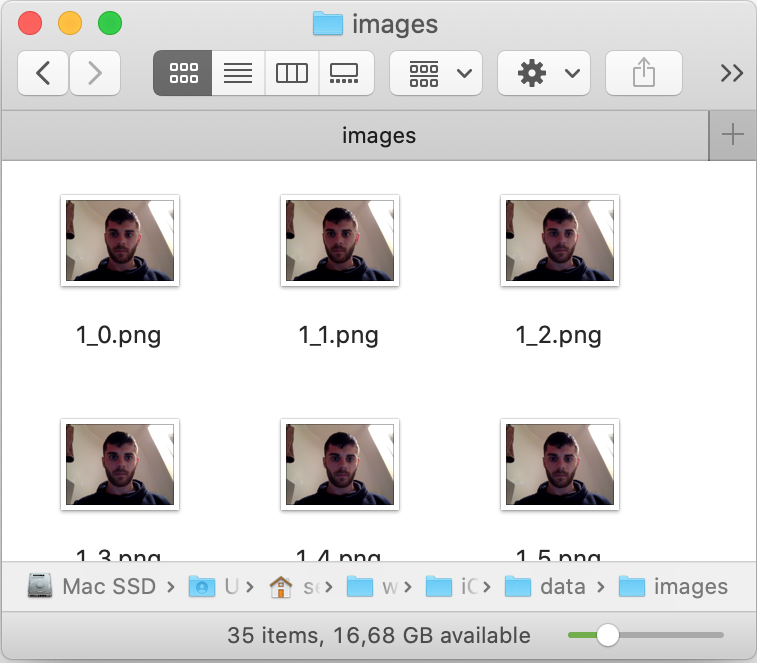
\includegraphics[width=0.3\textwidth]{data_structure_3.png}
    \caption{Cum am structurat datele}
\end{figure}

\begin{lstlisting}[language=Python, caption=Salvarea datelor]
def save_collected_data(self):
    if len(self.collected_data) == 0:
        return
    dc_logger.info(
        f'Acquiring lock for data collection. Locked = {self.collect_data_lock.locked()}')
    self.collect_data_lock.acquire()
    dc_logger.info('Lock acquired')
    session_no = self.get_session_number()
    dc_logger.info(f"Saving data for session_{session_no}")
    self.save_session_info(session_no)
    self.save_images_info(session_no)
    self.save_images(session_no)
    self.collect_data_lock.release()
    self.collected_data = []
    dc_logger.info('Saving data done')
\end{lstlisting}

% ~~~~~~~~~~ Data Collection Section ~~~~~~~~~~